\documentclass{beamer}

\usepackage[brazil]{babel}   
\usepackage[utf8]{inputenc} 
\usepackage{ragged2e} 

\newcommand{\er}{$\times$}

\mode<presentation>{ \usetheme{Copenhagen} \usecolortheme{seagull} }
\beamertemplatenavigationsymbolsempty

\setbeamertemplate{headline}
{%
\begin{beamercolorbox}{section in head/foot}
\vskip2pt\insertnavigation{\paperwidth}\vskip2pt
\end{beamercolorbox}%
}

\setbeamertemplate{footline}[frame number]
{
}

\title{Avaliação de desempenho de servidores de jogos cooperativos}
\subtitle{SSC-0142 Redes de Computadores}
\author{Lucas Junqueira Adami\inst{1}, Rafael Regis do Prado\inst{1}}
\institute
{
	\inst{1}
	Instituto de Ciências Matemáticas e de Computação -- Universidade de São Paulo\\
  	São Carlos, SP
}

\titlegraphic
{
	\includegraphics[scale=.2]{img/ICMC.jpg}\\
	\includegraphics[scale=.2]{img/LaSDPC.png}
}

\AtBeginSection[]
{
	\begin{frame}
    		\frametitle{Sumário}
    		\tableofcontents[currentsection]
  	\end{frame}
}

\begin{document}

\begin{frame}[plain]
	\titlepage
\end{frame}

\begin{frame}
    \frametitle{Sumário}
    \tableofcontents
\end{frame}
\section{Introdução}

\begin{frame} \frametitle{Introdução}
\begin{itemize}
	\item \justifying Em tarefas que são executadas em ambientes distintos a comunicação necessária para a interação dos nós envolvidos ocorre tipicamente por meio de uma rede;
	\item A eficiência da comunicação depende de muitos fatores:
	\begin{itemize}
		\item Congestionamento da rede;
		\item Qualidade do serviço de entrega de pacotes;
		\item Taxa de mensagens trocadas entre os computadores envolvidos.
	\end{itemize}
\end{itemize}
\end{frame}

\begin{frame} \frametitle{Introdução}
\begin{itemize}
	\item \justifying Em jogos cooperativos \textit{online} o maior foco está no tempo de resposta (atraso);
	\item É necessário padrões de comunicação entre os pares;
	\item \justifying Portanto, procura-se técnicas de transmissão de mensagens que sejam eficientes.
\end{itemize}
\end{frame}

\section{Objetivos}

\begin{frame} \frametitle{Objetivos}
\begin{itemize}
	\item \justifying Avaliar o desempenho dos diferentes modos de operação de \emph{sockets}:
	\begin{itemize}
		\item Bloqueante e não bloqueante;
		\item \emph{TCP} e \emph{UDP}.
	\end{itemize}
	\item \justifying Implementar um jogo cooperativo para os experimentos.
\end{itemize}	
\end{frame}

\section{Fundamentação Teórica}

\begin{frame} \frametitle{\emph{Sockets}}
\begin{itemize}
	\item \justifying \emph{Sockets} são definidos como interfaces que possibilitam o fluxo de dados entre dois nós por meio de uma rede, utilizando uma \emph{API} definida \cite{Tanenbaum};
	\item Eles operam sob dois modos:
	\begin{itemize}
		\item Bloqueante
		\item Não Bloqueante
	\end{itemize}
	\item \justifying \emph{Sockets} ainda utilizam dois protocolos da camada de transporte:
	\begin{itemize}
		\item \emph{TCP}
		\item \emph{UDP}
	\end{itemize}
\end{itemize}
\end{frame}

\section{Atividades Desenvolvidas}

\begin{frame} \frametitle{Planejamento do Experimento}
\begin{table}
  \center
  \tiny
  \begin{tabular}{|c|c|c|c|c|}
  \hline
    \#  & \textbf{Protocolo de transporte} & \textbf{Tipo de comunicação} & \textbf{Tamanho do pacote} & \textbf{Jogadores} \\ \hline
    1 & TCP & Não-bloqueante & 0 & 50 \\ \hline
    2 & TCP & Não-bloqueante & 0 & 100 \\ \hline
    3 & TCP & Não-bloqueante & 100 & 50 \\ \hline
    4 & TCP & Não-bloqueante & 100 & 100 \\ \hline
    5 & TCP & Bloqueante & 0 & 50 \\ \hline
    6 & TCP & Bloqueante & 0 & 100 \\ \hline
    7 & TCP & Bloqueante & 100 & 50 \\ \hline
    8 & TCP & Bloqueante & 100 & 100 \\ \hline
    9 & UDP & Não-bloqueante & 0 & 50 \\ \hline
    10 & UDP & Não-bloqueante & 0 & 100 \\ \hline
    11 & UDP & Não-bloqueante & 100 & 50 \\ \hline
    12 & UDP & Não-bloqueante & 100 & 100 \\ \hline
    13 & UDP & Bloqueante & 0 & 50 \\ \hline
    14 & UDP & Bloqueante & 0 & 100 \\ \hline
    15 & UDP & Bloqueante & 100 & 50 \\ \hline
    16 & UDP & Bloqueante & 100 & 100 \\ \hline
  \end{tabular} 
\caption{Experimentos planejados}
\label{tab:experimentos}
\end{table} 	
\end{frame}

\begin{frame} \frametitle{Configuração de Máquinas}
\begin{itemize}
	\item Nós Físicos:
	\begin{itemize}
  		\item Processador: Core2 Quad Q6600 8MB de Cache 2.40 Ghz;
  		\item Memória: 8GB DDR3 1333Mhz;
  		\item HD: Samsung 160GB Samsung 7200 RPM Sata II;
  		\item Rede: Gigabit Ethernet.
	\end{itemize}

	\item Nó Virtual:
	\begin{itemize}
  		\item Processador: 2 CPUs (2.40Ghz cada);
 		\item Memória: 4GB de RAM DDR3 1333 Mhz;
  		\item HD: Virtual de 15GB;
  		\item Rede: Gigabit Ethernet.
	\end{itemize}
\end{itemize}
\end{frame}

\begin{frame} \frametitle{Especificação do Protocolo}
\begin{table}
  \center
  \tiny
  \begin{tabular}{|c|c|c|c|}
  \hline
    \textbf{ID} & \textbf{Nome} & \textbf{Remetente} & \textbf{Campos (seguido do número de bytes)} \\ \hline
    0 & login & Cliente & Nome Jogador(20)  \\ \hline
    1 & add player & Servidor & Identificador(2), Coordenadas X e Y(4), Nome Jogador(20)\\ \hline
    2 & remove player & Servidor & Identificador(2) \\ \hline
    3 & move me & Cliente & Direção(1) (Ex: Norte=0, Leste=2) \\ \hline
    4 & move player & Servidor & Identificador(2), Coordenadas X e Y(4) \\ \hline
    5 & plant bomb & Cliente & \\ \hline
    6 & add bomb & Servidor &  Identificador(2), Coordenadas X e Y(4)  \\ \hline
    7 & explode bomb & Servidor & Identificador (2) \\ \hline
    8 & fall player & Servidor & Identificador (2) \\ \hline
    9 & acknowledge & Cliente & \\ \hline
   10 & ping & Cliente & \\ \hline
   11 & pong & Servidor & \\ \hline
   12 & info & Cliente & Média(16), Desvio Padrão(16), Pacotes Perdidos(4)  \\ \hline
   13 & shutdown & Servidor &\\ \hline
  \end{tabular} 
\caption{Protocolo do jogo criado}
\label{tab:protocolo}
\end{table} 
\end{frame}

\begin{frame} \frametitle{Desenvolvimento do Jogo Cooperativo}
\begin{itemize}
	\item \justifying Envolveu a implementação do servidor e a implementação do cliente;
	\item \justifying Utilizou-se \emph{C++} \cite{CPP} para a implementação do servidor e \emph{Java} \cite{Java} para a implementação dos
clientes;
	\item \justifying A ferramenta de versionamento \emph{Git} \cite{Git} foi escolhida como controladora de versão.
	\begin{itemize}
		\item \url{https://github.com/rafaelregis/bomberboys}
	\end{itemize}
\end{itemize}
\end{frame}

\begin{frame} \frametitle{Exemplo do Jogo}
\begin{figure}[ht]
  \centering
  \includegraphics[width=.7\textwidth]{img/partida.png}
  \caption{Exemplo de partida do jogo desenvolvido}
  \label{fig:partida}
\end{figure}
\end{frame}

\begin{frame} \frametitle{O Servidor}
\begin{figure}[ht]
  \centering
  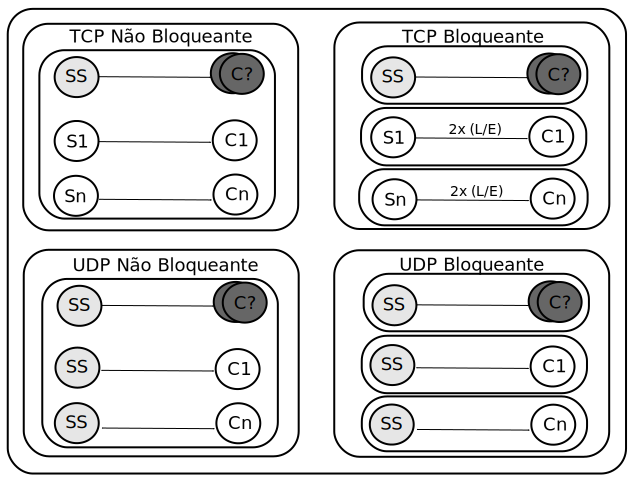
\includegraphics[width=.6\textwidth]{img/server.png}
  \caption{Modos de operação do servidor}
  \label{fig:server}
\end{figure}	
\end{frame}

\begin{frame} \frametitle{O Cliente}
\begin{itemize}
	\item \justifying Inicialização simultânea de um número variável de clientes;
	\item \justifying Conjunto de \textit{threads} para cada cliente e cada um se comunica com o servidor por seu próprio \textit{socket};
	\item \justifying Configuração do número de clientes, protocolo, modo de operação e tamanho da mensagem;
	\item \justifying Utilização de \emph{bots} para simular partida.
\end{itemize}
\end{frame}

\section{Resultados}

\begin{frame} \frametitle{Resultados}
\begin{table}
  \center
  \tiny
  \begin{tabular}{|c|c|c|c|c|c|}
  \hline
  \# & \textbf{Atraso ($ms$)} & \textbf{Variância ($ms$)} & \textbf{CPU (\%)} & \textbf{Bytes (enviado/recebido)} & \textbf{Pacotes Perdidos} \\ \hline
    1 & 50.04 & 1.74 & 16.1/9.6/73.6 & 21688636.2/438917162.9 & 0 \\ \hline
    2 & 302.68 & 192.15 & 27.8/7.2/63.83 & 21998667.43/380864913.9 & 0 \\ \hline
    3 & \er & \er & \er & \er & \er \\ \hline
    4 & \er & \er & \er & \er & \er \\ \hline
    5 & 50.16 & 3.14 & 31/25.6/43 & 20717318.5/310870796.8 & 0 \\ \hline
    6 & 53.89 & 12.08 & 33.15/31.5/34.75 & 35965675.65/375906838.45 & 0 \\ \hline
    7 & 50.02 & 0.53 & 23.4/44.2/32.2 & 66501124.9/2064695664.9 & 0 \\ \hline
    8 & 54.15 & 9.52 & 23.55/47.35/28.9 & 77556161.35/2327154624.80 & 0 \\ \hline
  \end{tabular} 
\caption{Resultados dos experimentos}
\label{tab:resultados}
\end{table}
\end{frame}

\begin{frame} \frametitle{Resultados}
\begin{figure}[ht]
  \centering
  \includegraphics[width=0.9\textwidth]{img/delay-graph.png}
  \caption{Tempos de atraso}
  \label{fig:delay-graph}
\end{figure}
\end{frame}

\begin{frame} \frametitle{Resultados}
\begin{figure}[ht]
  \centering
  \includegraphics[width=0.9\textwidth]{img/cpu-graph.png}
  \caption{Cargas de \emph{CPU}}
  \label{fig:cpu-graph}
\end{figure}
\end{frame}

\begin{frame} \frametitle{Resultados}
\begin{figure}[ht!]
  \centering
  \includegraphics[width=0.9\textwidth]{img/net-graph.png}
  \caption{\emph{Bytes} enviados e recebidos}
  \label{fig:net-graph}
\end{figure}
\end{frame}

\begin{frame} \frametitle{Resultados}
\begin{figure}[ht]
  \centering
  \includegraphics[width=0.9\textwidth]{img/tcp-graph.png}
  \caption{Tempos para o modo \emph{TCP} não bloqueante}
  \label{fig:tcp-graph}
\end{figure}
\end{frame}

\section{Conclusões}

\begin{frame} \frametitle{Conclusões}
\begin{itemize}
	\item \justifying \emph{UDP} de forma pura não pode ser aplicado para a comunicação entre cliente e servidor nesse contexto;
	\item \justifying O modo \emph{TCP} não bloqueante utiliza menos carga da \emph{CPU} e é mais fácil de programar;
	\item \justifying A partir de um número de clientes, a abordagem não bloqueante passou a gerar atrasos muito grandes. Portanto, é mais seguro utilizar a abordagem bloqueante, mais estável.
\end{itemize}	
\end{frame}

\section*{Referências}

\begin{frame}[allowframebreaks] \frametitle{Referências}
\bibliographystyle{apalike}
\bibliography{bibliography}
\end{frame}

\end{document}